\chapter{Análisis de Resultados}

%Section describiendo la simulación
%Geant4, ROOT y describiendo la geometría, las condiciones iniciales, materiales, etc.


\section{Configuración Perpendicular}
\subsection{Likelihood}
\begin{figure}
    \centering
    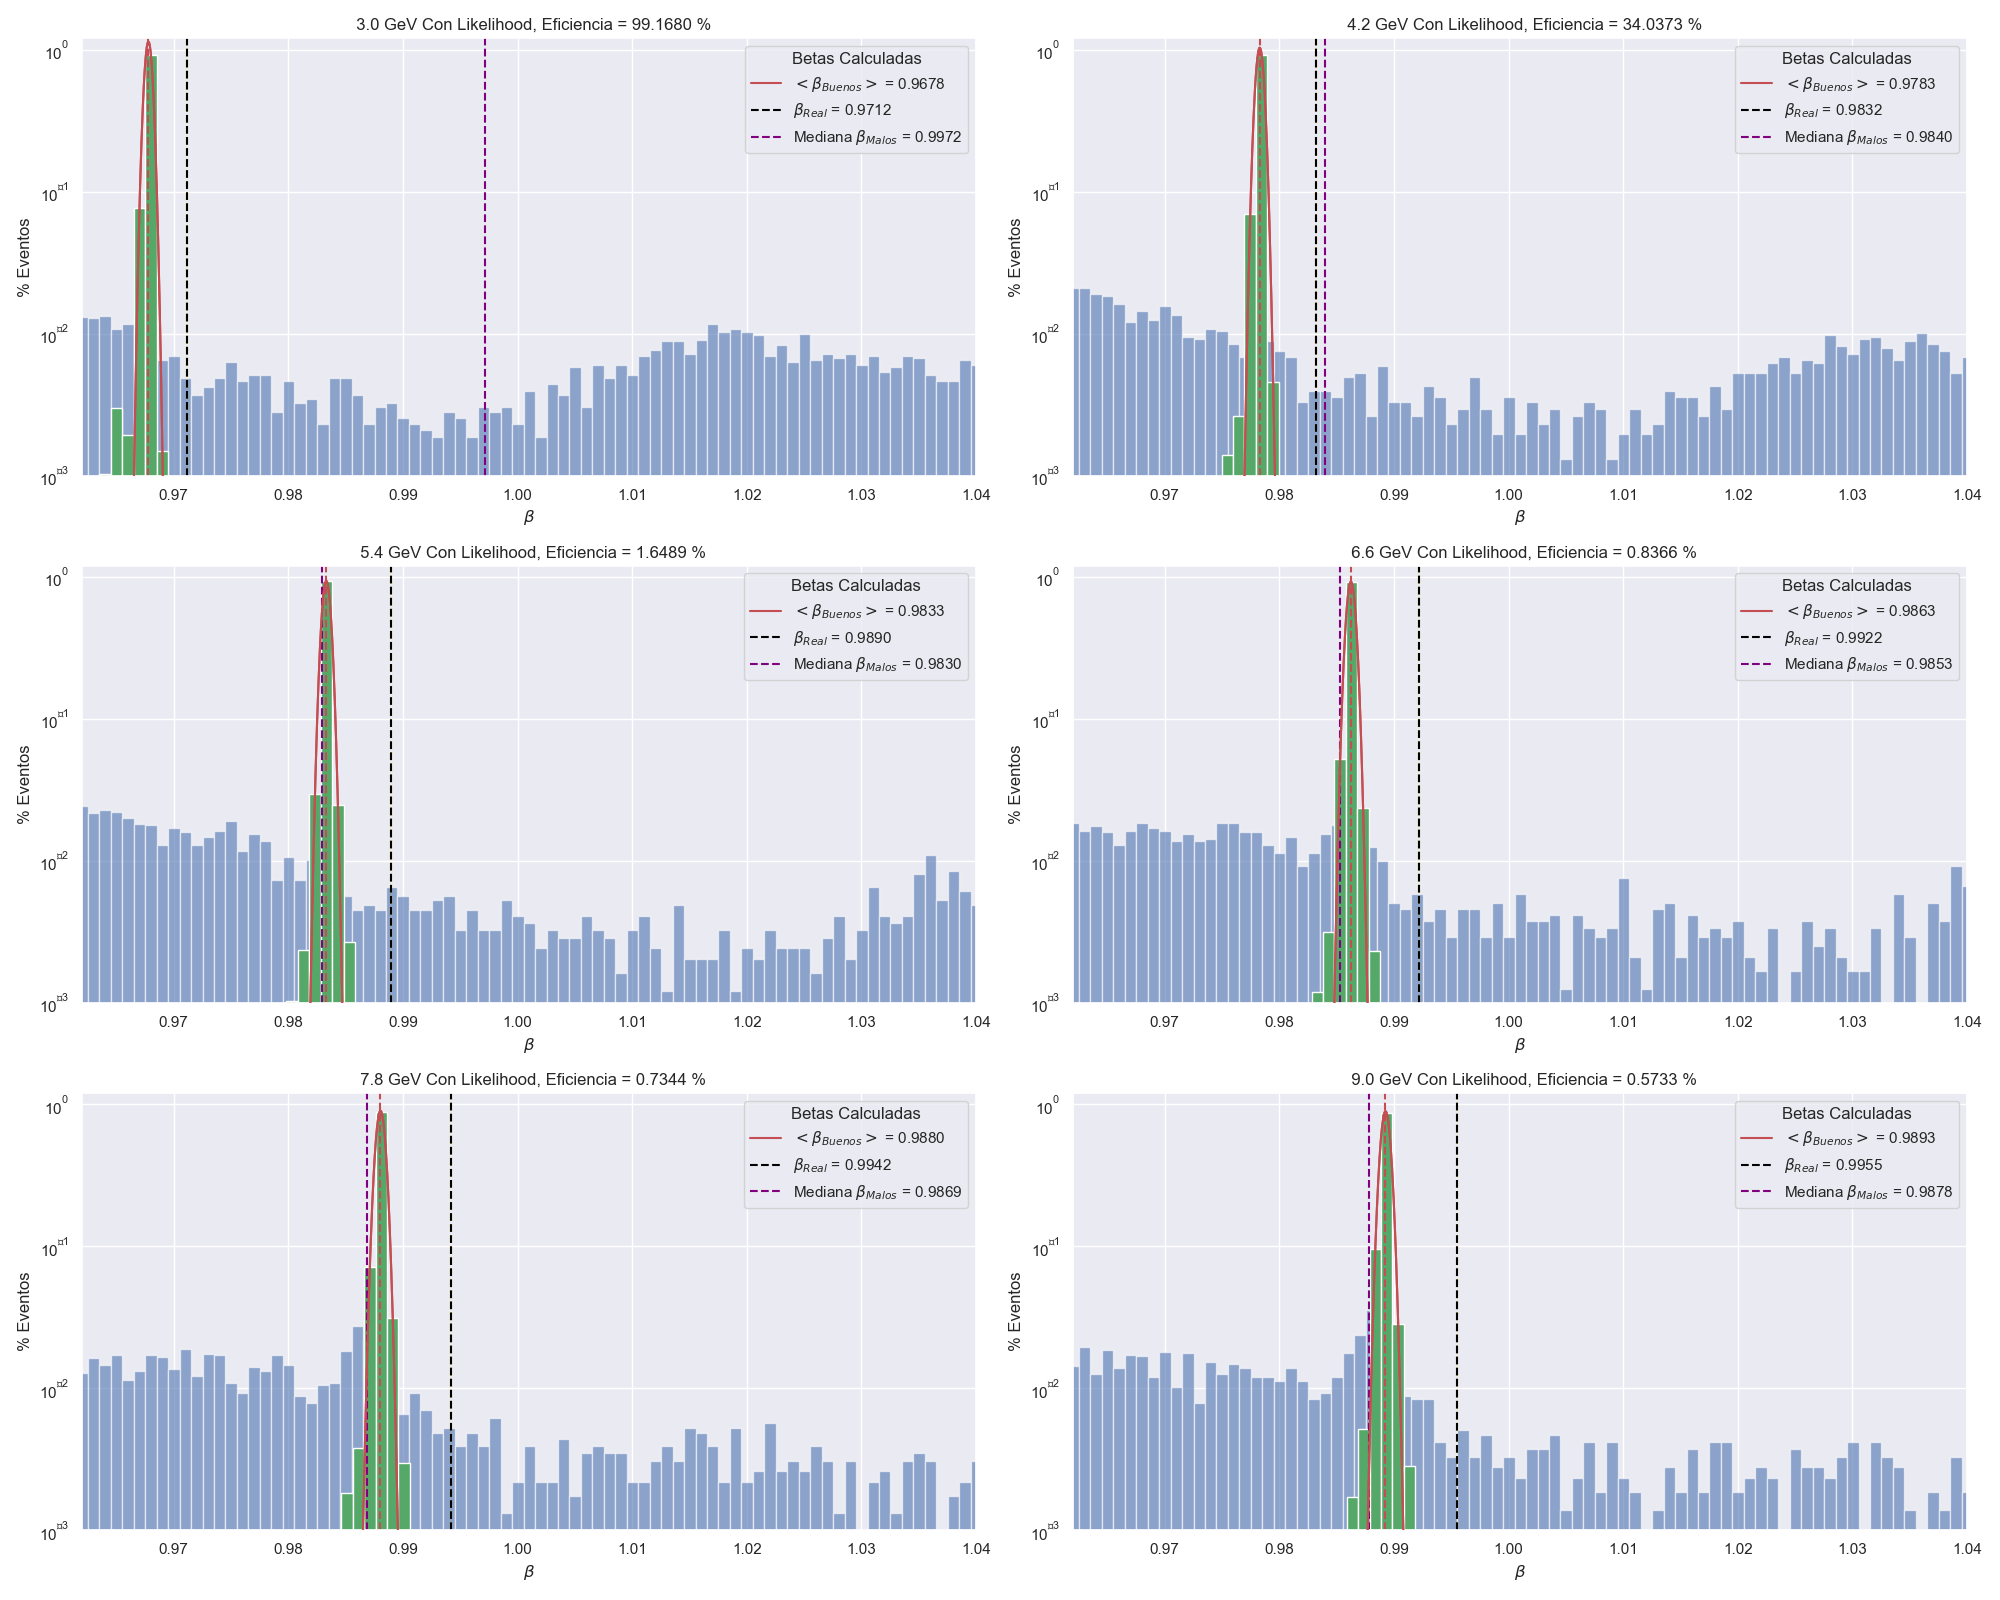
\includegraphics[width=18cm, height=21cm, left]{Tesis-UNAM/Capitulo4/pLike9.png}
    \caption{La eficiencia se refiere al porcentaje de eventos en el rango de 0.5\% con respecto a la beta real}
    \label{fig:enter-label}
\end{figure}

\boxed{$$f(x) = \begin{cases} 
          \frac{1}{\sigam 2\pi}exp\left( -\frac{1}{2}\frac{(x-\mu)^2}{\sigma^2} \right) & x \leq x_0 \\
           a_1\left(\frac{x}{x_0}\right)^{k_1} & x_0 \leq x\\
       \end{cases}
$$}

\begin{figure}
    \centering
    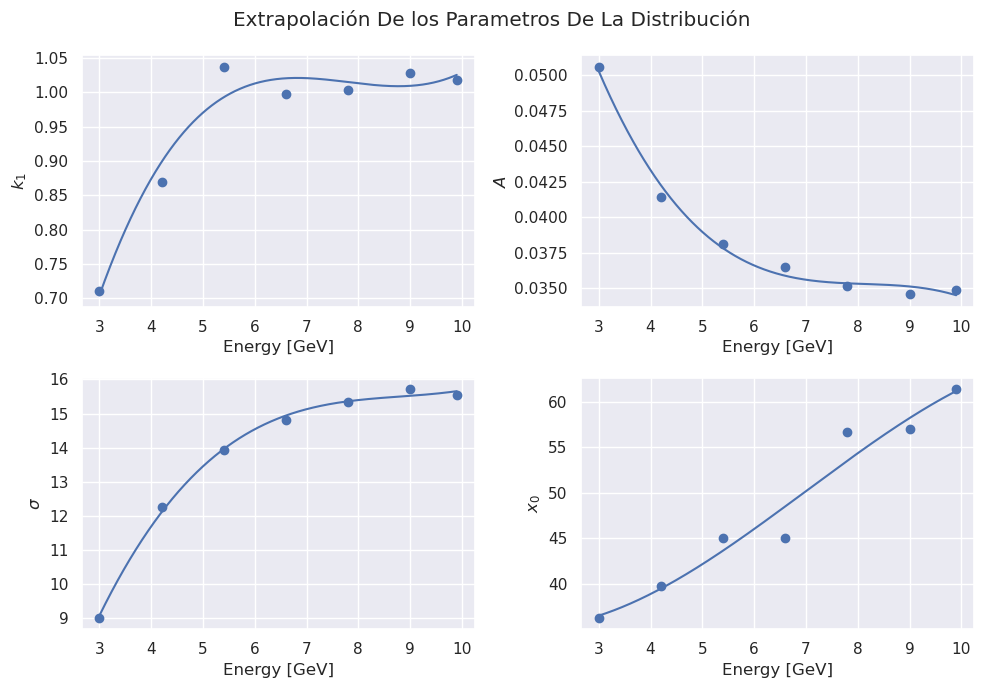
\includegraphics[width=12cm]{Tesis-UNAM/Capitulo4/parametros.png}
    \caption{Parámetros De La Distribución a Ajustar}
    \label{fig:enter-label}
\end{figure}

\begin{figure}
    \centering
    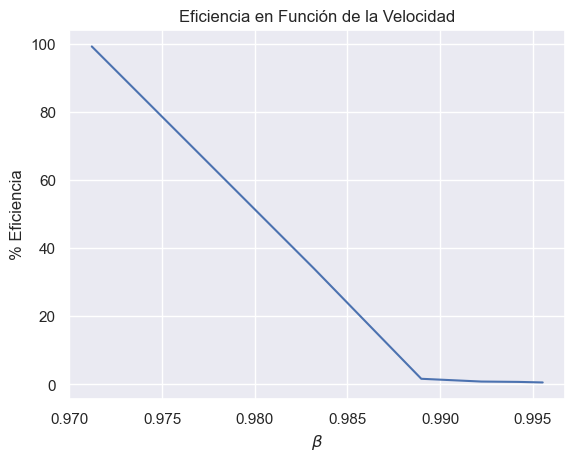
\includegraphics[scale=0.6]{Tesis-UNAM/Capitulo4/EficienciaLike.png}
    \caption{9cm Aerogel}
    \label{fig:enter-label}
\end{figure}

\begin{figure}
    \centering
    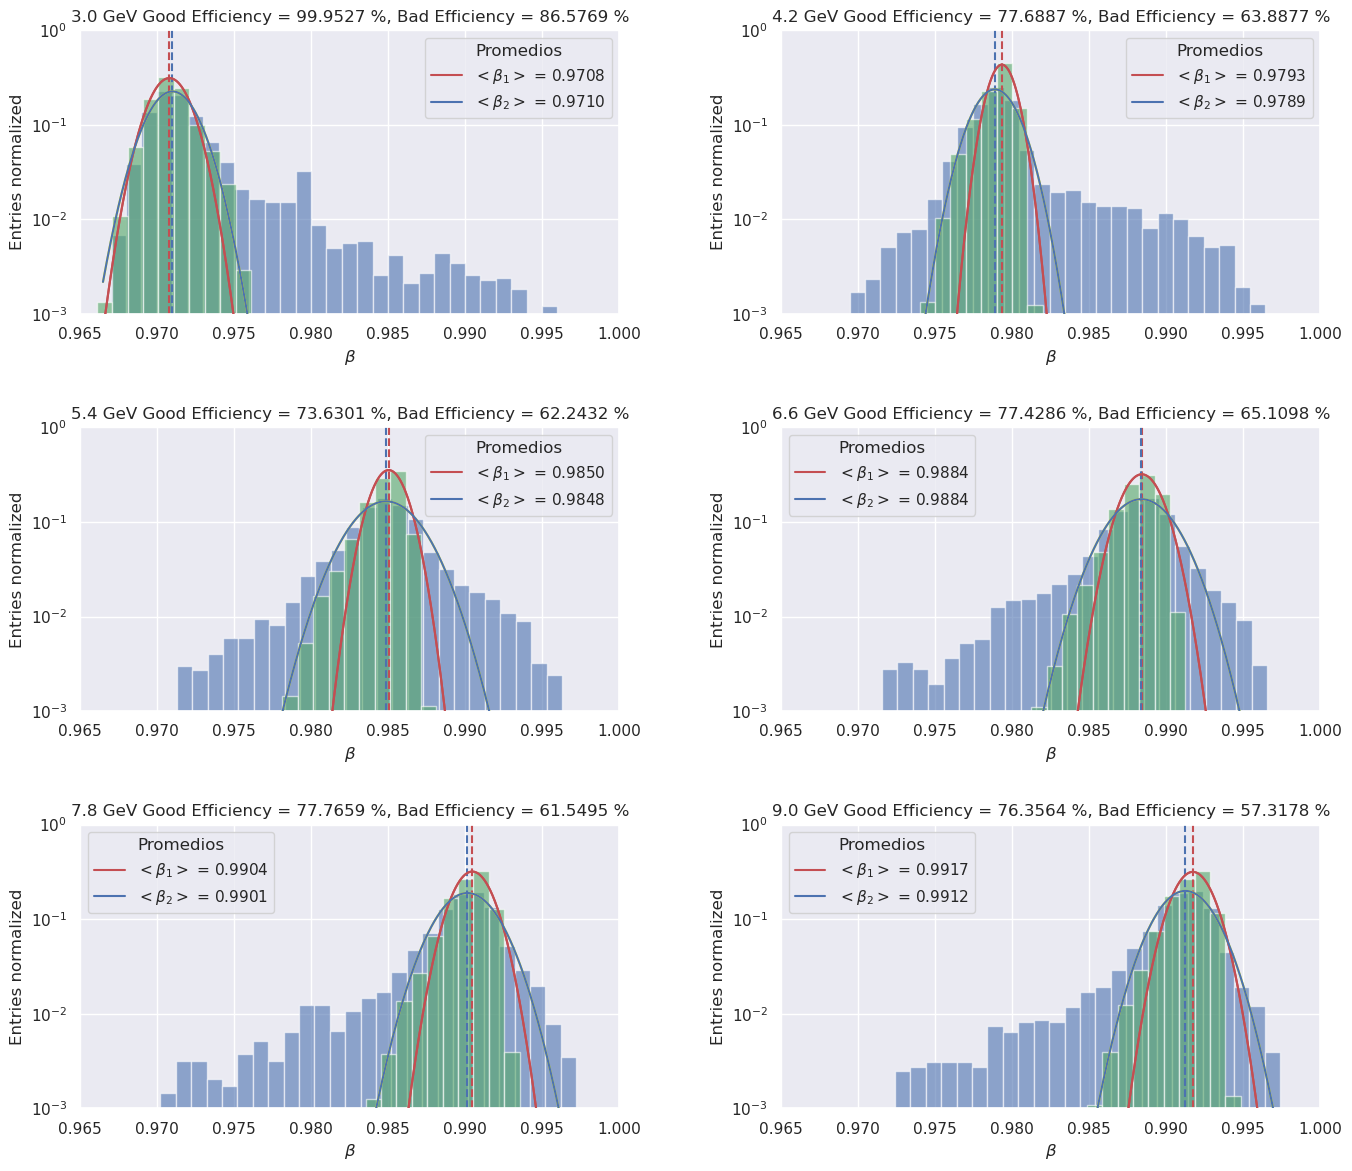
\includegraphics[width=15cm, height=21cm]{Tesis-UNAM/Capitulo4/9pAI.png}
    \caption{9cm Aerogel}
    \label{fig:enter-label}
\end{figure}

\begin{figure}
    \centering
    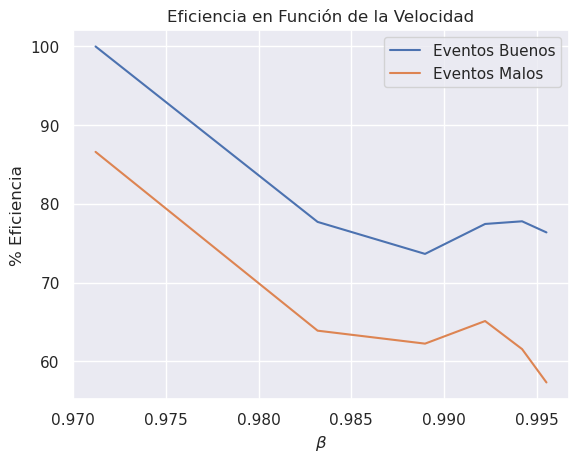
\includegraphics[scale=0.6]{Tesis-UNAM/Capitulo4/EficienciaAI.png}
    \caption{9cm Aerogel}
    \label{fig:enter-label}
\end{figure}
\subsection{Redes Neuronales}
\subsection{Comparación}
\section{Configuración Multidireccional}
\subsection{Likelihood}
\subsection{Redes Neuronales}
\subsection{Comparación}